\newpage
\subsection{Diseño de base de datos}

El sistema utiliza una estructura lógica común para representar las entidades principales del dominio, tanto en la base local SQLite como en la base central en la nube. La diferencia entre ambos entornos no radica principalmente en el modelo de datos, sino en el alcance de los registros almacenados. La base local SQLite conserva únicamente la información necesaria para que el dispositivo móvil opere sin conexión, mientras que la base en la nube concentra los registros sincronizados desde los distintos dispositivos asociados a las cuentas.

Debido al enfoque \textit{offline-first}, los registros generados en la aplicación móvil se almacenan inicialmente en SQLite y posteriormente se sincronizan hacia la nube cuando existe conexión a internet. 

Para conservar la trazabilidad, los identificadores generados localmente se mantienen durante la sincronización, permitiendo que un mismo registro tenga la misma identidad lógica en ambos entornos.

\subsubsection{Modelo entidad-relación}

El \textit{Modelo Entidad-Relación (MER)} es una representación conceptual de la estructura de datos de un sistema, utilizada para identificar las entidades que lo conforman, sus atributos y las relaciones que existen entre ellas. Su propósito es modelar la información que el sistema necesita almacenar de forma organizada, independientemente de la tecnología de base de datos que se utilice para su implementación. En el MER, las entidades representan objetos del mundo real con existencia propia, los atributos describen sus características y las relaciones expresan cómo se vinculan entre sí.

El modelo entidad-relación del presente sistema está conformado por seis entidades principales que reflejan los elementos operativos del proceso de monitoreo forestal. La entidad \textbf{cuenta} identifica a los usuarios del sistema y su rol, mientras que la entidad \textbf{dispositivo} registra los equipos móviles autorizados para operar con la aplicación móvil. La vinculación entre ambas se gestiona mediante la entidad \textbf{cuenta\_dispositivo}, que controla qué dispositivos están asociados a cada cuenta y su estado de asociación.

En cuanto a la información operativa, la entidad \textbf{árbol} almacena los registros individuales del arbolado monitoreado, y la entidad \textbf{zona\_follaje} registra las áreas geográficas identificadas mediante análisis macro. Ambas se relacionan con la entidad \textbf{análisis}, que concentra los resultados de clasificación obtenidos a partir de las imágenes capturadas, diferenciando entre análisis de corteza a nivel de árbol individual y análisis de follaje a nivel de zona. Finalmente, la entidad \textbf{análisis\_cromático} complementa cada análisis almacenando los porcentajes de coloración obtenidos mediante OpenCV, correspondientes a los rangos de evidencia visual definidos por la NOM-019-SEMARNAT-2017 \cite{nom019_semarnat_2017}.


\begin{figure}[H]
    \centering
    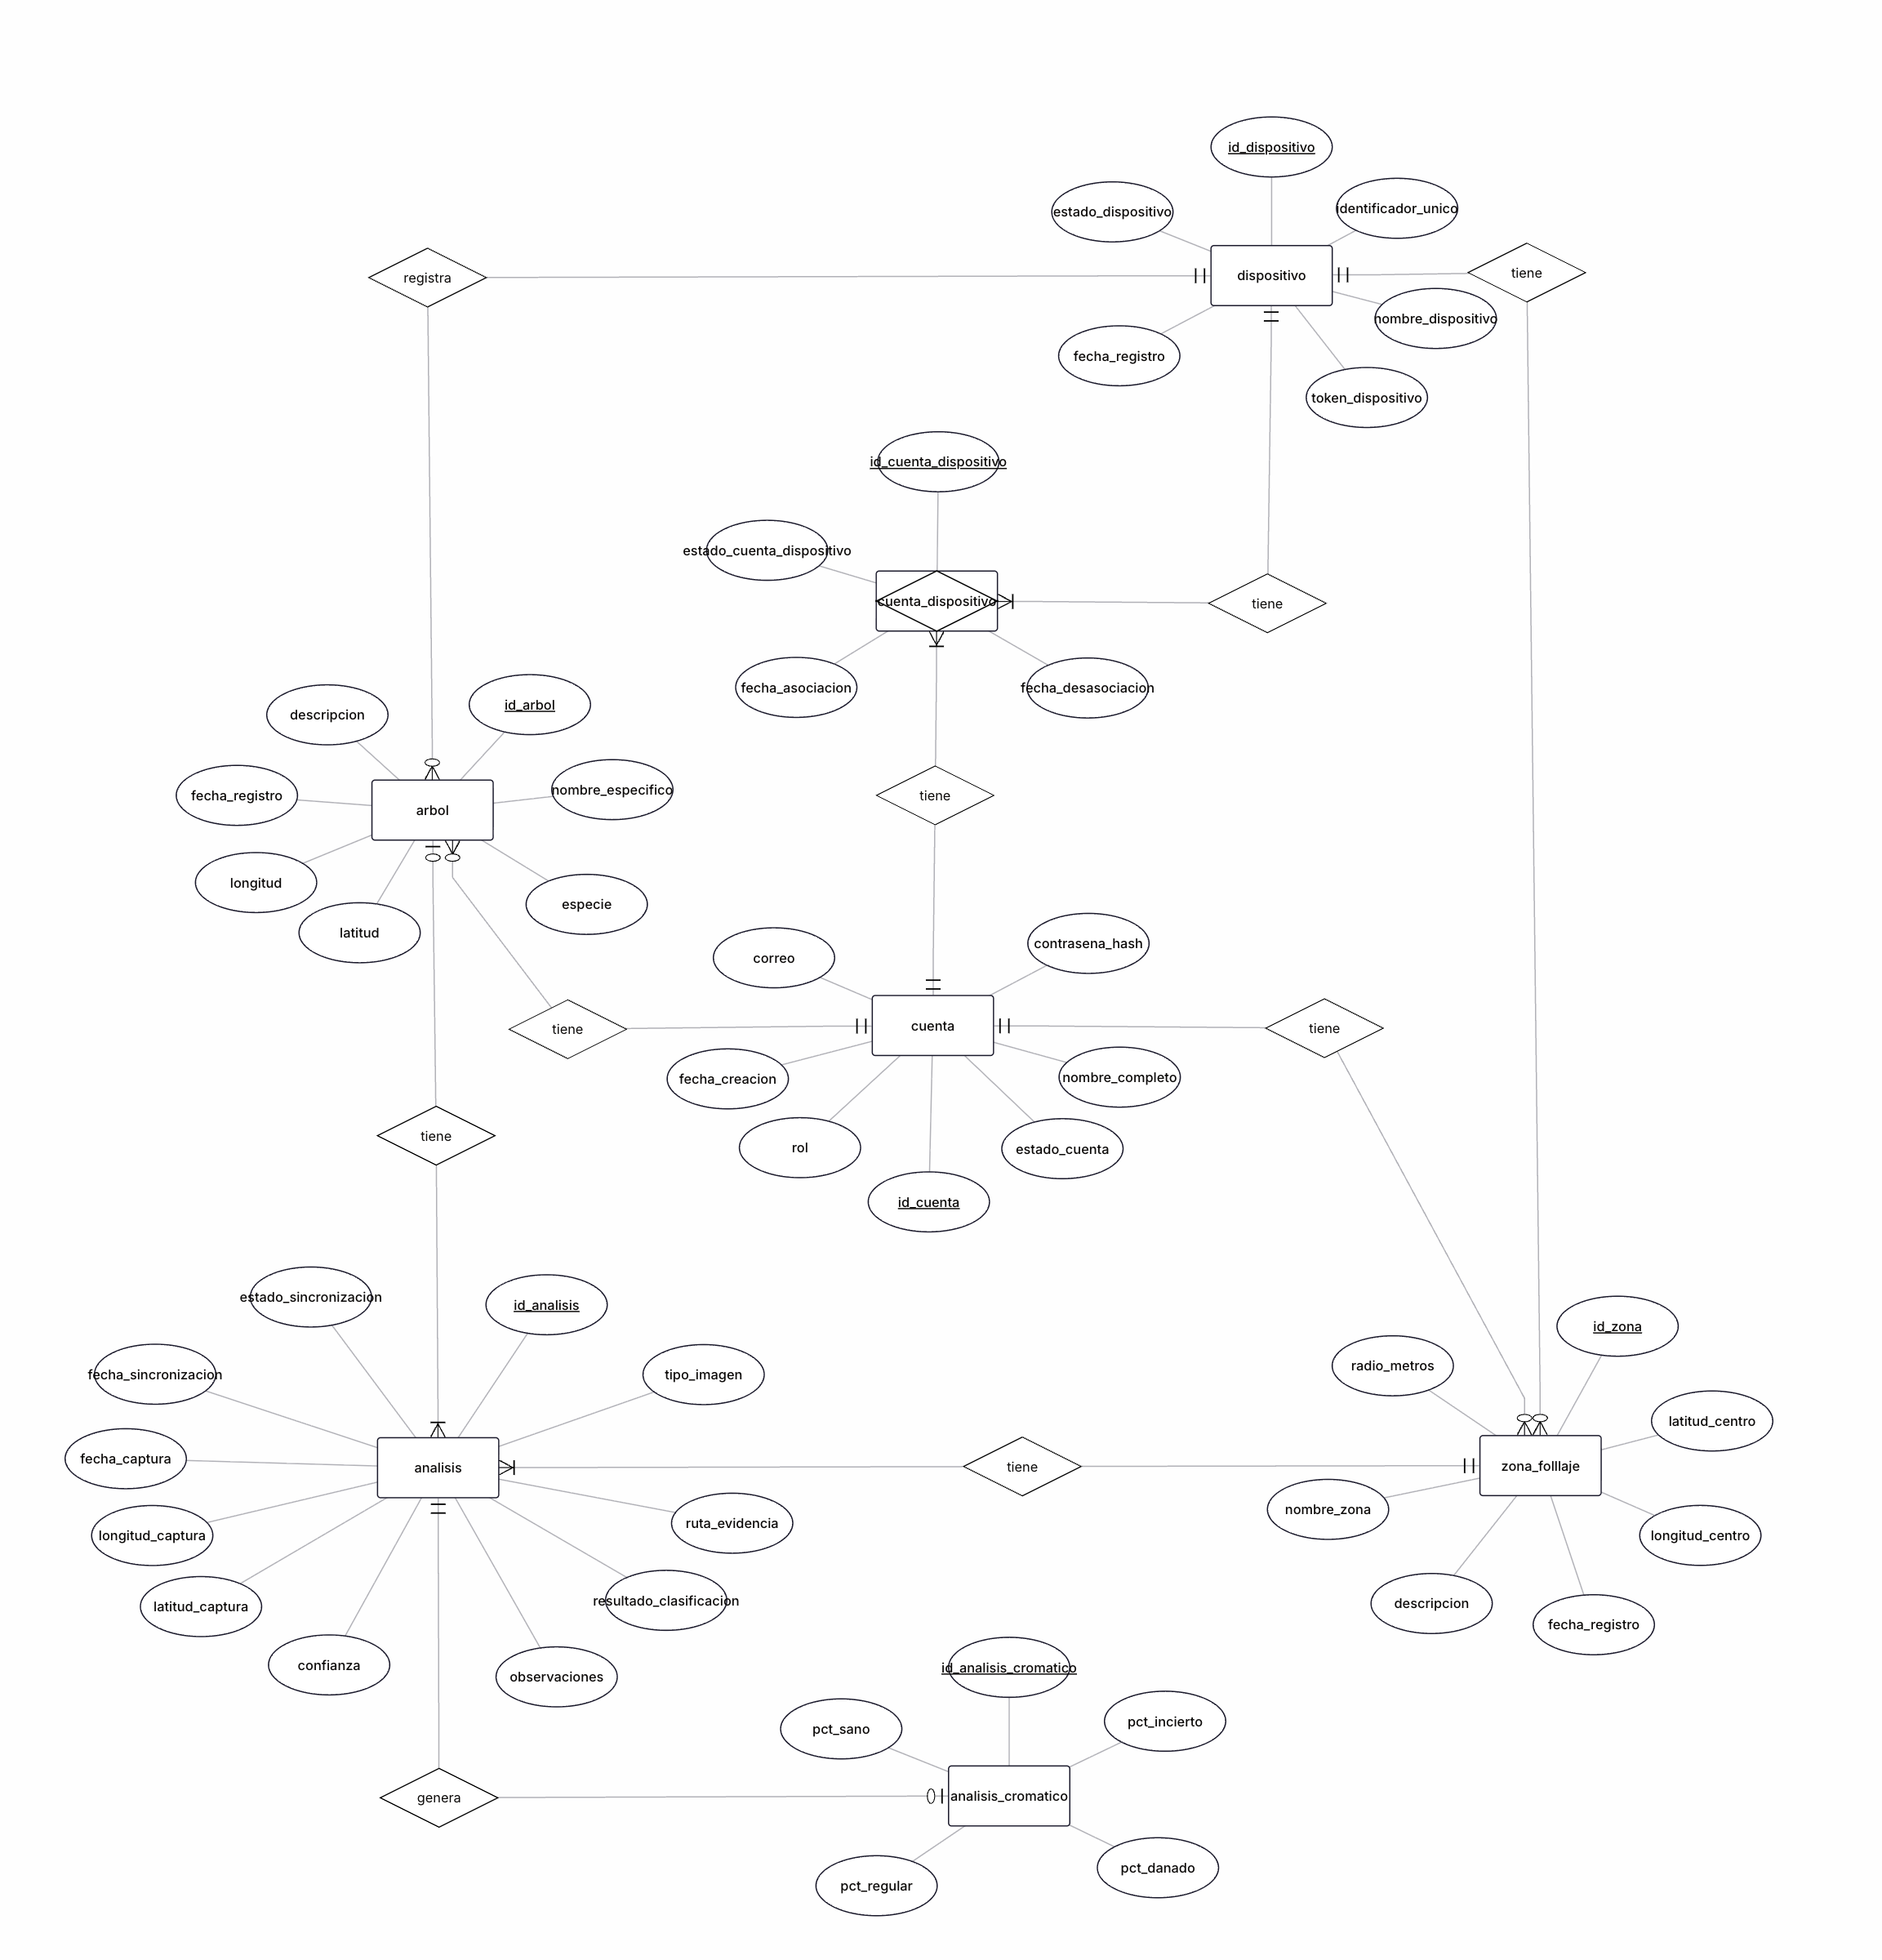
\includegraphics[width=0.9\textwidth]{images/C8/mer.png}
    \caption{MER: Sistema móvil y web}
\end{figure}

\subsubsection{Esquema relacional}

El \textit{esquema relacional} es la representación lógica de la base de datos derivada del modelo entidad-relación, expresada en términos de tablas, columnas, claves primarias y claves foráneas. A diferencia del MER, el esquema relacional está orientado a la implementación, definiendo con precisión cómo se organizan y vinculan los datos dentro del gestor de base de datos.

El esquema relacional del sistema se deriva del modelo entidad-relación y está conformado por siete tablas principales: \textbf{CUENTA}, \textbf{DISPOSITIVO}, \textbf{CUENTA\_DISPOSITIVO}, \textbf{ARBOL}, \textbf{ZONA\_FOLLAJE}, \textbf{ANALISIS} y \textbf{ANALISIS\_CROMATICO}. Estas tablas permiten representar tanto la gestión de usuarios y dispositivos como los registros operativos generados durante el monitoreo forestal.

Las tablas \textbf{CUENTA}, \textbf{DISPOSITIVO} y \textbf{CUENTA\_DISPOSITIVO} concentran la información de autenticación, autorización y asociación de dispositivos móviles. Por su parte, \textbf{ARBOL} y \textbf{ZONA\_FOLLAJE} representan las entidades monitoreadas según el tipo de captura realizada: corteza para árboles individuales y follaje para zonas geográficas.

La tabla \textbf{ANALISIS} almacena los resultados de cada captura, incluyendo la referencia de la evidencia, coordenadas de captura, resultado de clasificación, confianza y estado de sincronización. Esta tabla se asocia de forma condicional con \textbf{ARBOL} o \textbf{ZONA\_FOLLAJE}, dependiendo de si el análisis corresponde a corteza o follaje. Finalmente, \textbf{ANALISIS\_CROMATICO} almacena los porcentajes derivados del análisis complementario de color asociado a cada análisis.

\begin{figure}[H]
    \centering
    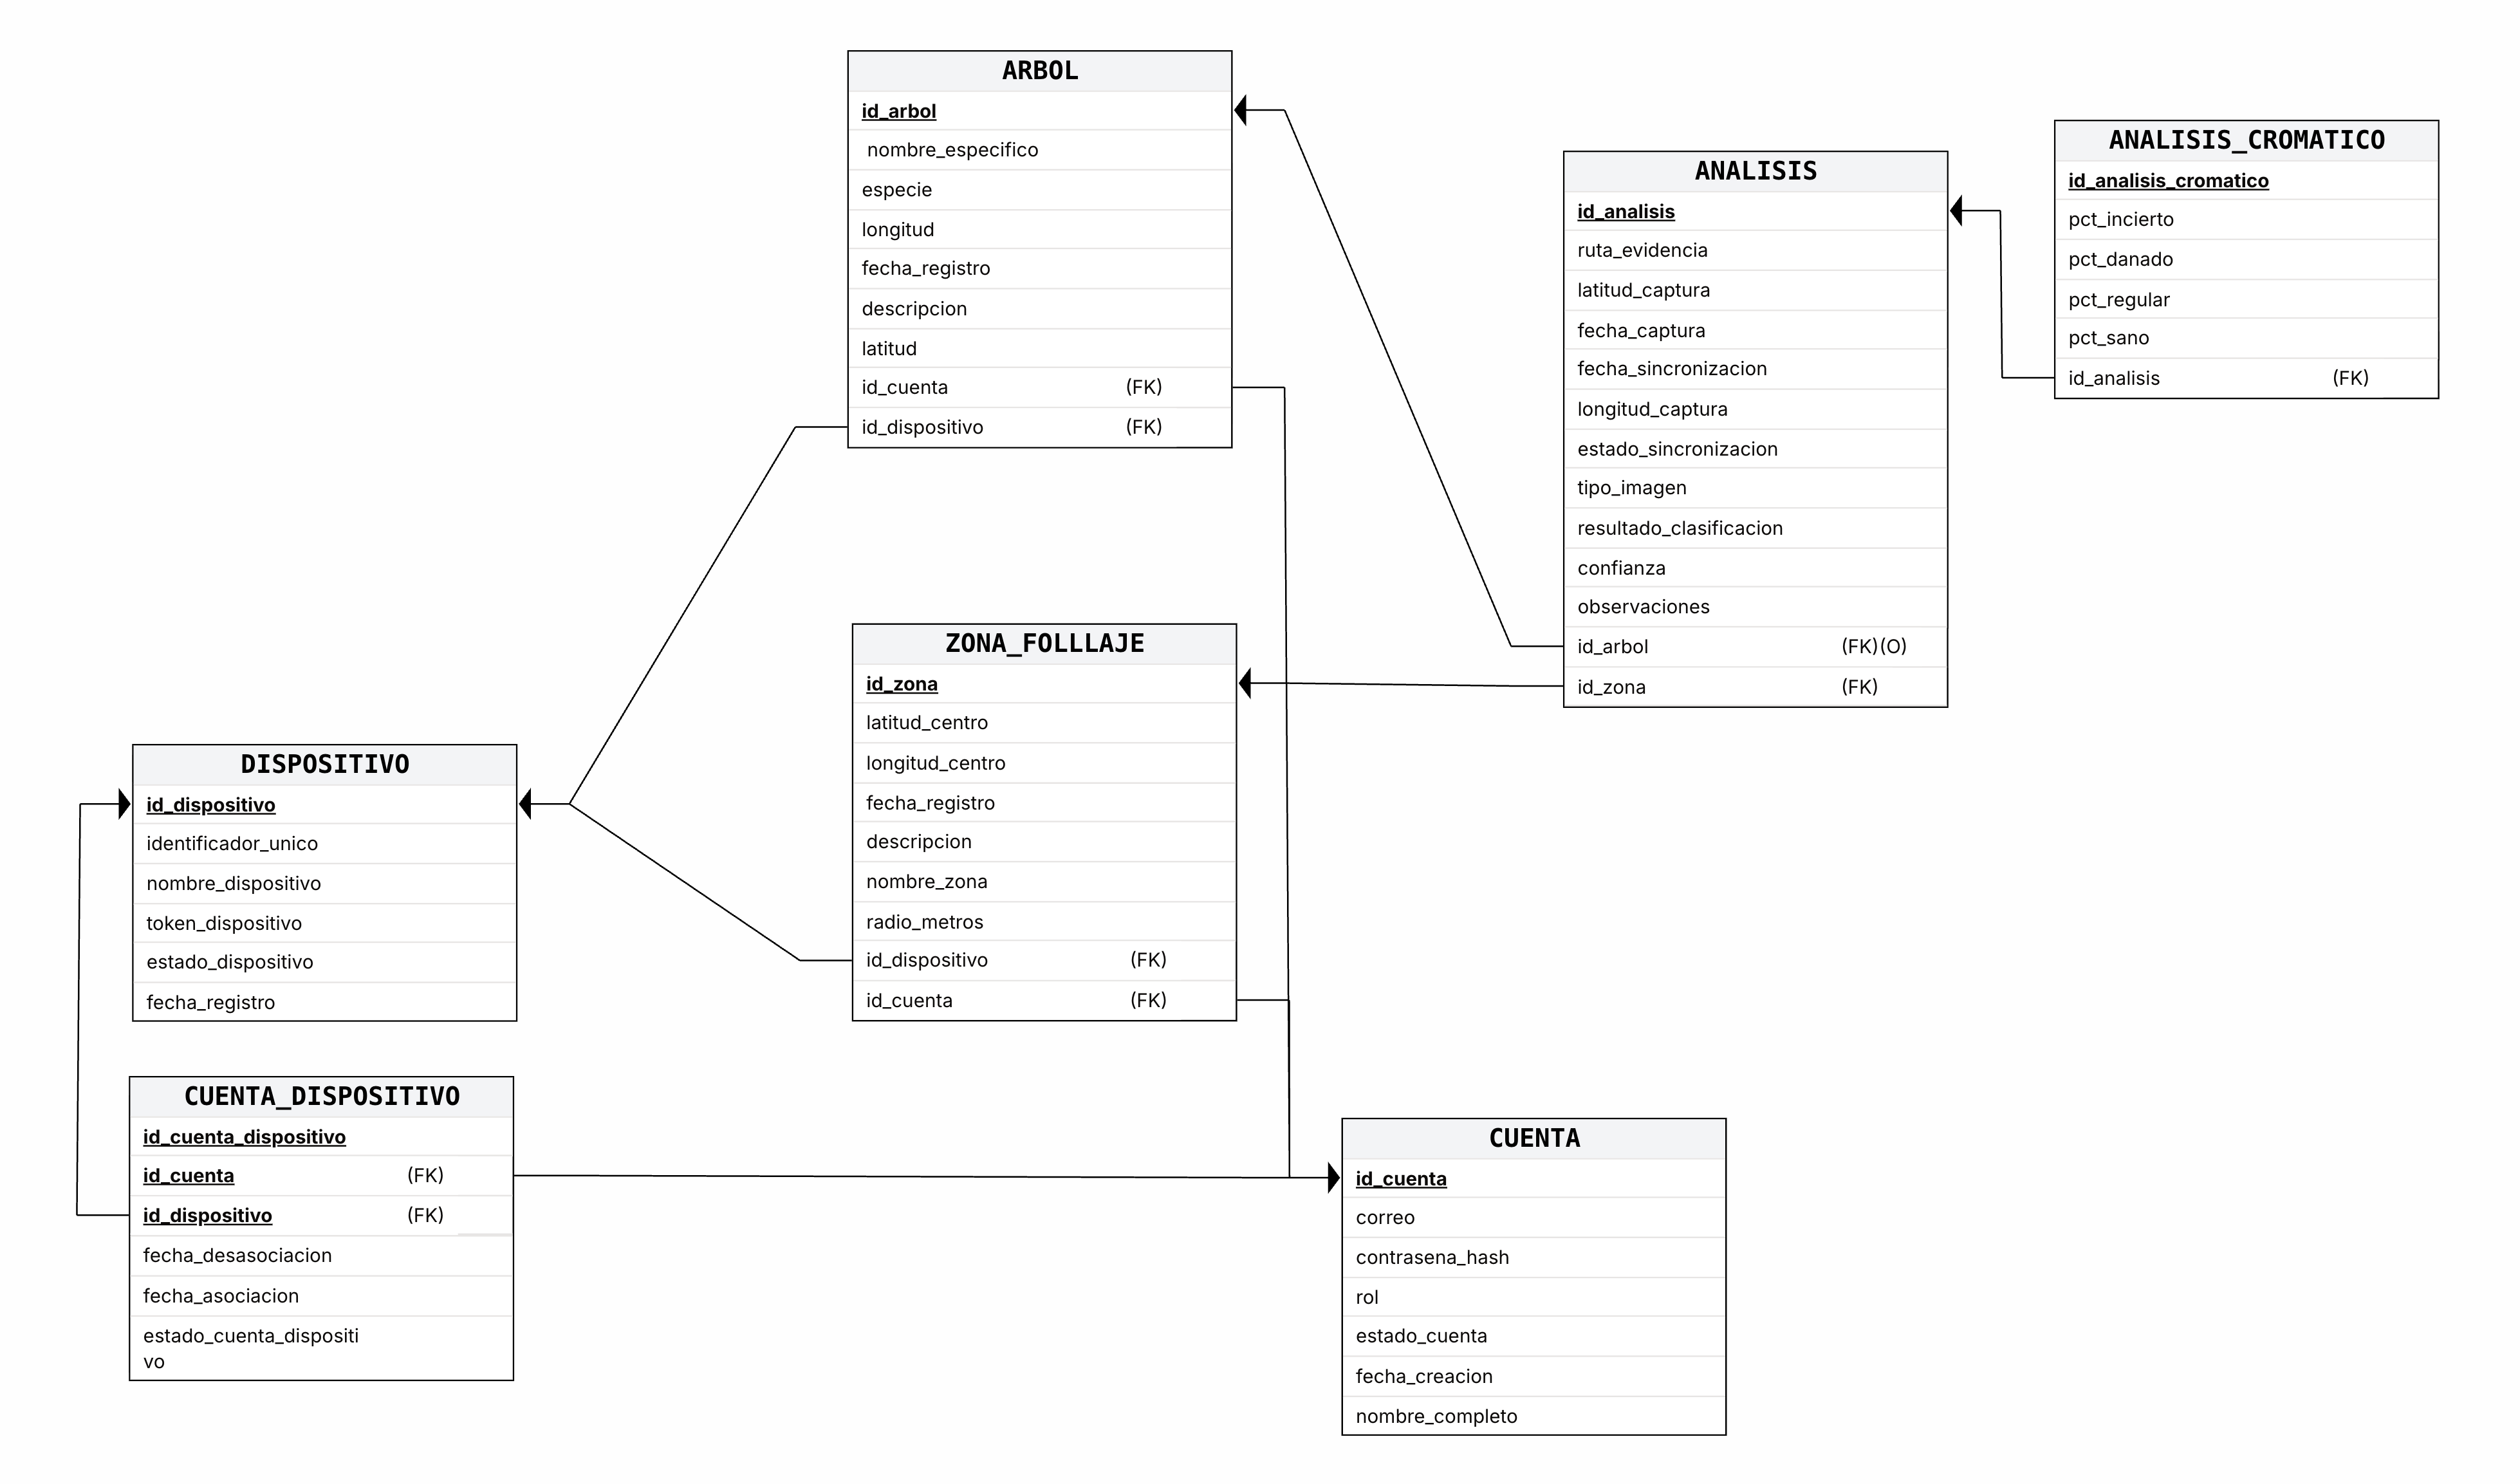
\includegraphics[width=1\textwidth]{images/C8/er.png}
    \caption{ER: Sistema móvil y web}
\end{figure}


\subsubsection{Diccionario de datos}

El diccionario de datos describe los atributos que integran cada tabla del esquema relacional, indicando su significado, tipo de dato sugerido, restricciones y función dentro del sistema. Esta sección complementa el modelo entidad-relación y el esquema relacional, ya que detalla la forma en que se almacenan e interpretan los datos utilizados por la aplicación móvil y la plataforma web.

%---------------------------------------
% TABLA: CUENTA
%---------------------------------------

\begin{longtable}{|>{\centering\arraybackslash}m{3cm}|>{\centering\arraybackslash}m{2.5cm}|m{8cm}|}
\caption{Diccionario de datos de la tabla CUENTA}\label{tab:dicCuenta} \\
\hline
\textbf{Campo} & \textbf{Tipo} & \textbf{Descripción} \\
\hline
\endfirsthead

\multicolumn{3}{c}%
{{\bfseries Tabla \thetable\ -- continuación}} \\
\hline
\textbf{Campo} & \textbf{Tipo} & \textbf{Descripción} \\
\hline
\endhead

id\_cuenta & UUID & Identificador único de la cuenta. Corresponde a la clave primaria de la tabla. \\
\hline
correo & VARCHAR & Correo electrónico utilizado para iniciar sesión en el sistema. Debe ser único. \\
\hline
contrasena\_hash & VARCHAR & Contraseña cifrada o hasheada de la cuenta. No se almacena en texto plano. \\
\hline
rol & VARCHAR & Rol asignado a la cuenta. Puede corresponder a Experto de campo o Administrador. \\
\hline
estado\_cuenta & VARCHAR & Estado actual de la cuenta, por ejemplo: activa o desactivada. \\
\hline
fecha\_creacion & TIMESTAMP & Fecha y hora en que la cuenta fue registrada en el sistema. \\
\hline
nombre\_completo & VARCHAR & Nombre completo del usuario asociado a la cuenta. \\
\hline

\end{longtable}

%---------------------------------------
% TABLA: DISPOSITIVO
%---------------------------------------

\begin{longtable}{|>{\centering\arraybackslash}m{3cm}|>{\centering\arraybackslash}m{2.5cm}|m{8cm}|}
\caption{Diccionario de datos de la tabla DISPOSITIVO}\label{tab:dicDispositivo} \\
\hline
\textbf{Campo} & \textbf{Tipo} & \textbf{Descripción} \\
\hline
\endfirsthead

\multicolumn{3}{c}%
{{\bfseries Tabla \thetable\ -- continuación}} \\
\hline
\textbf{Campo} & \textbf{Tipo} & \textbf{Descripción} \\
\hline
\endhead

id\_dispositivo & UUID & Identificador único del dispositivo. Corresponde a la clave primaria de la tabla. \\
\hline
identificador\_unico & VARCHAR & Identificador técnico del dispositivo móvil, utilizado para reconocer el equipo autorizado. \\
\hline
nombre\_dispositivo & VARCHAR & Nombre descriptivo del dispositivo, asignado para facilitar su identificación. \\
\hline
token\_dispositivo & VARCHAR & Token asociado al dispositivo, utilizado para identificación técnica o notificaciones. \\
\hline
estado\_dispositivo & VARCHAR & Estado del dispositivo dentro del sistema, por ejemplo: activo, inactivo o bloqueado. \\
\hline
fecha\_registro & TIMESTAMP & Fecha y hora en que el dispositivo fue registrado en el sistema. \\
\hline

\end{longtable}

%---------------------------------------
% TABLA: CUENTA_DISPOSITIVO
%---------------------------------------

\begin{longtable}{|>{\centering\arraybackslash}m{3.5cm}|>{\centering\arraybackslash}m{2.5cm}|m{7.5cm}|}
\caption{Diccionario de datos de la tabla CUENTA\_DISPOSITIVO}\label{tab:dicCuentaDispositivo} \\
\hline
\textbf{Campo} & \textbf{Tipo} & \textbf{Descripción} \\
\hline
\endfirsthead

\multicolumn{3}{c}%
{{\bfseries Tabla \thetable\ -- continuación}} \\
\hline
\textbf{Campo} & \textbf{Tipo} & \textbf{Descripción} \\
\hline
\endhead

id\_cuenta\_dispositivo & UUID & Identificador único de la asociación entre una cuenta y un dispositivo. Corresponde a la clave primaria. \\
\hline
id\_cuenta & UUID & Clave foránea que referencia a la cuenta asociada. \\
\hline
id\_dispositivo & UUID & Clave foránea que referencia al dispositivo asociado. \\
\hline
fecha\_asociacion & TIMESTAMP & Fecha y hora en que el dispositivo fue asociado a la cuenta. \\
\hline
fecha\_desasociacion & TIMESTAMP & Fecha y hora en que el dispositivo fue desasociado de la cuenta, si aplica. \\
\hline
estado\_cuenta\_dispositivo & VARCHAR & Estado de la relación entre cuenta y dispositivo, por ejemplo: activa o desasociada. \\
\hline

\end{longtable}

%---------------------------------------
% TABLA: ARBOL
%---------------------------------------

\begin{longtable}{|>{\centering\arraybackslash}m{3cm}|>{\centering\arraybackslash}m{2.5cm}|m{8cm}|}
\caption{Diccionario de datos de la tabla ARBOL}\label{tab:dicArbol} \\
\hline
\textbf{Campo} & \textbf{Tipo} & \textbf{Descripción} \\
\hline
\endfirsthead

\multicolumn{3}{c}%
{{\bfseries Tabla \thetable\ -- continuación}} \\
\hline
\textbf{Campo} & \textbf{Tipo} & \textbf{Descripción} \\
\hline
\endhead

id\_arbol & UUID & Identificador único del árbol registrado. Corresponde a la clave primaria de la tabla. \\
\hline
nombre\_especifico & VARCHAR & Nombre o identificador descriptivo asignado al árbol por el Experto de campo. \\
\hline
especie & VARCHAR & Especie o tipo de árbol registrado, en caso de ser conocida. \\
\hline
longitud & FLOAT & Coordenada geográfica de longitud correspondiente a la ubicación general del árbol. \\
\hline
latitud & FLOAT & Coordenada geográfica de latitud correspondiente a la ubicación general del árbol. \\
\hline
fecha\_registro & TIMESTAMP & Fecha y hora en que el árbol fue registrado en el sistema. \\
\hline
descripcion & TEXT & Información adicional u observaciones generales sobre el árbol registrado. \\
\hline
id\_cuenta & UUID & Clave foránea que referencia la cuenta a la que pertenece el árbol. \\
\hline
id\_dispositivo & UUID & Clave foránea que referencia el dispositivo desde el cual se registró el árbol. \\
\hline

\end{longtable}

%---------------------------------------
% TABLA: ZONA_FOLLAJE
%---------------------------------------

\begin{longtable}{|>{\centering\arraybackslash}m{3cm}|>{\centering\arraybackslash}m{2.5cm}|m{8cm}|}
\caption{Diccionario de datos de la tabla ZONA\_FOLLAJE}\label{tab:dicZonaFollaje} \\
\hline
\textbf{Campo} & \textbf{Tipo} & \textbf{Descripción} \\
\hline
\endfirsthead

\multicolumn{3}{c}%
{{\bfseries Tabla \thetable\ -- continuación}} \\
\hline
\textbf{Campo} & \textbf{Tipo} & \textbf{Descripción} \\
\hline
\endhead

id\_zona & UUID & Identificador único de la zona de follaje. Corresponde a la clave primaria de la tabla. \\
\hline
latitud\_centro & FLOAT & Latitud del punto central de la zona de follaje. \\
\hline
longitud\_centro & FLOAT & Longitud del punto central de la zona de follaje. \\
\hline
fecha\_registro & TIMESTAMP & Fecha y hora en que la zona fue registrada o generada. \\
\hline
descripcion & TEXT & Descripción general de la zona de follaje. \\
\hline
nombre\_zona & VARCHAR & Nombre descriptivo asignado a la zona para facilitar su identificación. \\
\hline
radio\_metros & FLOAT & Radio aproximado de cobertura de la zona, expresado en metros. \\
\hline
id\_dispositivo & UUID & Clave foránea que referencia el dispositivo desde el cual se registró la zona. \\
\hline
id\_cuenta & UUID & Clave foránea que referencia la cuenta a la que pertenece la zona. \\
\hline

\end{longtable}

%---------------------------------------
% TABLA: ANALISIS
%---------------------------------------

\begin{longtable}{|>{\centering\arraybackslash}m{3.2cm}|>{\centering\arraybackslash}m{2.5cm}|m{7.8cm}|}
\caption{Diccionario de datos de la tabla ANALISIS}\label{tab:dicAnalisis} \\
\hline
\textbf{Campo} & \textbf{Tipo} & \textbf{Descripción} \\
\hline
\endfirsthead

\multicolumn{3}{c}%
{{\bfseries Tabla \thetable\ -- continuación}} \\
\hline
\textbf{Campo} & \textbf{Tipo} & \textbf{Descripción} \\
\hline
\endhead

id\_analisis & UUID & Identificador único del análisis realizado. Corresponde a la clave primaria de la tabla. \\
\hline
ruta\_evidencia & VARCHAR & Ruta relativa de la imagen asociada al análisis. En SQLite referencia el archivo temporal local; en la nube referencia la evidencia almacenada remotamente. \\
\hline
latitud\_captura & FLOAT & Latitud exacta desde donde se realizó la captura del análisis. \\
\hline
longitud\_captura & FLOAT & Longitud exacta desde donde se realizó la captura del análisis. \\
\hline
fecha\_captura & TIMESTAMP & Fecha y hora en que se realizó la captura de la imagen. \\
\hline
fecha\_sincronizacion & TIMESTAMP & Fecha y hora en que el análisis fue sincronizado con la nube. Puede estar vacío mientras el registro esté pendiente. \\
\hline
estado\_sincronizacion & VARCHAR & Estado del proceso de sincronización del análisis, por ejemplo: pendiente, sincronizado o error. \\
\hline
tipo\_imagen & VARCHAR & Tipo de imagen analizada. Puede corresponder a follaje o corteza. \\
\hline
resultado\_clasificacion & VARCHAR & Resultado obtenido por el modelo de clasificación o análisis aplicado a la imagen. \\
\hline
confianza & FLOAT & Nivel de confianza asociado al resultado de clasificación. \\
\hline
observaciones & TEXT & Comentarios u observaciones agregadas por el Experto de campo. \\
\hline
id\_arbol & UUID & Clave foránea opcional hacia la tabla ARBOL. Se utiliza cuando el análisis corresponde a corteza. \\
\hline
id\_zona & UUID & Clave foránea opcional hacia la tabla ZONA\_FOLLAJE. Se utiliza cuando el análisis corresponde a follaje. \\
\hline

\end{longtable}

%---------------------------------------
% TABLA: ANALISIS_CROMATICO
%---------------------------------------

\begin{longtable}{|>{\centering\arraybackslash}m{3.5cm}|>{\centering\arraybackslash}m{2.5cm}|m{7.5cm}|}
\caption{Diccionario de datos de la tabla ANALISIS\_CROMATICO}\label{tab:dicAnalisisCromatico} \\
\hline
\textbf{Campo} & \textbf{Tipo} & \textbf{Descripción} \\
\hline
\endfirsthead

\multicolumn{3}{c}%
{{\bfseries Tabla \thetable\ -- continuación}} \\
\hline
\textbf{Campo} & \textbf{Tipo} & \textbf{Descripción} \\
\hline
\endhead

id\_analisis\_cromatico & UUID & Identificador único del análisis cromático. Corresponde a la clave primaria de la tabla. \\
\hline
pct\_incierto & FLOAT & Porcentaje de la imagen clasificado como incierto dentro del análisis cromático. \\
\hline
pct\_danado & FLOAT & Porcentaje de la imagen clasificado como dañado. \\
\hline
pct\_regular & FLOAT & Porcentaje de la imagen clasificado como regular. \\
\hline
pct\_sano & FLOAT & Porcentaje de la imagen clasificado como sano. \\
\hline
id\_analisis & UUID & Clave foránea que referencia el análisis al que pertenece el análisis cromático. \\
\hline

\end{longtable}

En la tabla \textbf{ANALISIS}, los campos \textbf{id\_arbol} e \textbf{id\_zona} se consideran condicionales. Cuando el análisis corresponde a corteza, el registro se asocia a un árbol mediante \textbf{id\_arbol} y \textbf{id\_zona} permanece vacío. Cuando el análisis corresponde a follaje, el registro se asocia a una zona mediante \textbf{id\_zona} y \textbf{id\_arbol} permanece vacío. Esta decisión permite utilizar una sola tabla de análisis para representar ambos tipos de captura sin duplicar estructuras.